\documentclass[conference]{IEEEtran}
\IEEEoverridecommandlockouts
% The preceding line is only needed to identify funding in the first footnote. If that is unneeded, please comment it out.
\usepackage{cite}
\usepackage{amsmath,amssymb,amsfonts}
\usepackage{algorithmic}
\usepackage{graphicx}
\usepackage{textcomp}
\usepackage{xcolor}
\def\BibTeX{{\rm B\kern-.05em{\sc i\kern-.025em b}\kern-.08em
    T\kern-.1667em\lower.7ex\hbox{E}\kern-.125emX}}
\begin{document}

\section{Overview of Key Elements in Big Data Systems}

The primary objective of this section is to delineate the crucial constituents of big data systems. The components under consideration are derived from the systematic literature review (SLR) as referenced by \cite{b1} and \cite{b2}, complemented by a brief literary review of the existing knowledge.

Reference architectures presented in \cite{b1} and \cite{b2} were assessed and juxtaposed to pinpoint recurrent elements in big data architectural references. While some ARs, being brief, offered minimal insights, others, like NIST, were notably exhaustive. A prevailing observation was the tendency of ARs to be rooted in existing knowledge, substantiating the idea that crafting ARs from a foundation of pre-existing knowledge can be more potent than starting afresh.

In a systematic pursuit of this inquiry and subsequent to our data collation, we enumerated all the elements from every big data AR discussed prior. These elements find their description in Table 2. One challenge was the variation in terminologies used across different studies to delineate architectural components. While architectural definition languages, like Archimate, find limited adoption, most researchers resort to bespoke ontologies using simple diagrams. This renders comparison challenging, often necessitating translation from one conceptual framework to another.

An automated textual assessment was initially conducted on the naming of these components, aiming to discern trends and word preferences. The graphical representation of these terminologies is illustrated in Figure 3. Notably, terms such as ‘big data application provider’ and ‘big data framework provider’ emerged as common nomenclatures, possibly attributed to the influence of NIST BD AR. Universally accepted terms included ‘data consumer’ and ‘data provider’, with ‘layer’ being the chosen descriptor for logically segmenting various AR components.

Distilling the above, to aptly address RQ2, we meticulously analyzed these components and sorted them based on functionality into: 1) Big Data Management and Storage, 2) Data Processing and Interface Applications, 3) Big Data Infrastructure.

\subsection{Big Data Management and Storage}


The inherent diversity of data is one of big data's quintessential hallmarks. This multifaceted nature of data necessitates the exploration and adoption of a variety of storage methodologies. An apt exemplification of this trend is the use of 'polyglot persistence'. In contexts where real-time and high-performance data is paramount, databases like ScyllaDB - renowned for their ultra-low latency and scalability - emerge as the optimal choice. Conversely, for scenarios demanding intricate relationships between data entities, the prowess of modern non-relational databases other than Neo4J, such as ArangoDB with its multi-model capabilities, becomes evident.

Selecting an appropriate database, or even multiple databases, embodies a pivotal architectural choice. This decision extends beyond mere storage, affecting patterns of data access and caching. For instance, in the realm of distributed systems specializing in micro-services architecture, many professionals are leaning towards the Command Query Responsibility Segregation (CQRS) pattern, known for bolstering the efficiency of event-driven applications. Two essential cornerstones of big data architectures are undeniably the storage type and its associated access pattern.

However, the prevailing sentiment in big data reference architectures (BD RAs) is an inclination towards monolithic storage strategies, epitomized by data warehouses and data lakes. While the conventional model of data staging and storage within data warehouses might seem ill-equipped to manage extensive big data volumes, it's intriguing to note the persistence of such methodologies in some modern proposals. A noteworthy element in many BD RAs is the data lake concept. Essentially, a data lake acts as a repository capable of accommodating a plethora of data forms, both internal and external. Data is typically fetched from these lakes to undergo transformation, a process delineated as LET (load, extract, transform), contrasting the older ETL (extract, transform, load) technique.

Drawing parallels between Business Intelligence (BI) and big data, one notices stark contrasts in the nature of their source data. In a similar vein, data lakes and data warehouses exhibit distinct characteristics. Traditional data warehouses predominantly rely on relational databases, which might restrict analytical flexibility and surge operational costs. Data lakes, however, offer a reservoir to store diverse data without pre-defined schemas, enhancing adaptability. Yet, this adaptability isn't without pitfalls. The unchecked dumping of data into lakes, disregarding its organization and consumption patterns, might inadvertently morph these lakes into inaccessible data swamps. Implementing data governance and proactive metadata can be potential antidotes to such scenarios.

Synthesizing the above, it's apparent that BD RAs are anchored in three dominant paradigms:

\begin{enumerate}
    \item Enterprise data warehouse model.
    \item     Data lake model.
    \item     Multi-modal cloud-based model.
\end{enumerate}

While the enterprise data warehouse model leans heavily on monolithic structures with ETLs and established data processing pathways, the data lake model resonates with a later-stage data processing approach. The third, cloud-centric paradigm seamlessly integrates distributed systems’ elements and cloud functionalities. Some RAs discussed in \cite{b1} operate at an elevated abstraction layer, making it challenging to infer storage natures or data pipeline characteristics. One good example of such RAs is the NIST BD RA \cite{b3}.

Yet, a broad spectrum of concerns often goes unaddressed in the realm of big data management. Critical areas like security, privacy, metadata management, and data quality sometimes appear sidelined. The scalability of some RAs in light of burgeoning data sources and their adaptability to evolving regional data privacy mandates also remain subjects of scrutiny. Discussions encapsulating data architecture, discoverability, and interoperability are conspicuously absent. 

\subsection{Data Handling and Interface Architectures}

Big Data (BD) systems commonly navigate through two primary data handling realms: stream and batch processing. Stream processing, also known as rapid processing, addresses urgent tasks like identifying potentially fraudulent credit card activity. On the other hand, batch processing takes its time, ideal for in-depth analyses such as regression studies.

In Big Data systems, the decision between stream or batch processing is primarily dictated by the three V's of data: variety, volume, and velocity.

Variety refers to the many forms of data, ranging from structured data like databases to unstructured data such as text or images. Stream processing might handle a diverse set of live data feeds, such as social media posts, sensor data from IoT devices, or real-time e-commerce transactions. These data types necessitate different processing paradigms. An algorithm sifting through real-time tweets to gauge sentiment would require an entirely different setup than one analyzing images from surveillance cameras to detect anomalies.

Volume alludes to the sheer amount of data. In scenarios with massive influxes of data, stream processing, utilizing technologies like Apache Kafka or Apache Flink, can offer real-time insights without storing vast quantities of information first. Conversely, batch processing is beneficial for situations where large chunks of accumulated data need comprehensive analysis. Consider the example of log files accumulated over a month from a popular application. Analyzing this data for patterns, anomalies, or insights would typically employ batch processing methods. Tools like Apache Hadoop or Apache Spark's batch processing capabilities can process this vast data efficiently.

Velocity pertains to the speed at which new data is generated and collected. High-velocity scenarios, such as stock trading platforms, necessitate stream processing for near-instantaneous responses. Here, technologies like Storm or Flink, which are designed for high-speed data inflows, become crucial. They can, for instance, quickly analyze patterns to inform immediate trading decisions. On the other hand, in cases where data arrives at a more steady and predictable rate, batch processing methods using techniques like MapReduce or BSP would be more apt. An example here might be the monthly sales data from a chain of retail stores, where data is accumulated over a more extended period and then processed to derive insights for the next month.

To add another layer of complexity, certain scenarios merge both processing modes. A hybrid approach, known as the Lambda architecture, combines the latency benefits of stream processing with the thoroughness and accuracy of batch processing. For instance, a weather forecasting system might employ stream processing to provide immediate weather updates from live sensors and batch processing to analyze historical data and refine its forecasting models.

The literature presents various layers of granularity when discussing data handling. While certain studies delve deep into the intricacies of the data handling pipeline, others simplify it to terms like 'batch' or 'stream' processing.

Furthermore, we discerned two main approaches to data handling. One methodology integrates both batch and stream processing within a singular architectural frame, while the other differentiates between the two. This distinction is evident in the Lambda and Kappa architectural philosophies and their derived RAs. Some RAs even introduce a triad: the batch node, streaming node, and interactive node.

In terms of BD interface communication, two patterns emerge. Some RAs showcase a simple 'access layer'. Others present multifaceted components tailored to unique needs, such as Machine Learning (ML) or Business Intelligence (BI). Moreover, succesfully approaches of software engineering such as domain-driven design and micro-services patterns are being progressingly applied to the realm of data engineering. One good example of this is the study conducted in \cite{b4} and data mesh \cite{b5}.

\subsection{Data Infrastructure Considerations in Big Data Architectures}

Infrastructure, an essential facet discussed across various Reference Architectures (RAs), exhibits variation in its depiction among different authors. While some delineate this component using standard architectural description languages, others imply its presence subtly without direct specification. Some architectures even delve deeply into both infrastructure and platform layers.

A salient component in the NIST Big Data RA is the "big data framework provider," which covers aspects such as computing, analytics, data organization, distribution, and key infrastructures like networking, computing, and storage.

It's more apt to conceptualize the Big Data (BD) infrastructure as a foundational layer, sketching out the possible computing and networking architecture for a Big Data system. Given the industry's tilt towards distributed paradigms and horizontal scaling, this layer's significance surges. This landscape prompts architects to grapple with challenges tied to the CAP theorem, ACID and BASE transactions, data consistency, service discovery, and tail latency. This raises the question: Should the Big Data system be event-driven, leveraging platforms like Kafka? Or should it remain anchored to REST-based communication? A pivotal concern also lies in understanding the overhead implications of context switches and inter-service networking.

Gleaning insights from our Systematic Literature Review (SLR), we observed the BD infrastructure surfacing in a myriad of forms and methodologies. While one could argue that infrastructure is an inherent component across various systems, its design nuances are particularly accentuated in BD systems due to their characteristic distributed nature.

A dimension that often slips through the cracks is DataOps. Despite its transformative potential in seamlessly automating and delivering data engineering tasks, its presence seems sparse in many Big Data RAs. Another revelation is that not every RA fully harnesses the benefits of comprehensive distributed architectures, even though Big Data systems could greatly capitalize on this design approach. An exception to this trend heavily borrows from the patterns of event-driven microservices architecture. Figure~\ref{BDcomponents} portrayes the high-level overview of the BD components discussed.

\begin{figure}[h!]
    \centering
    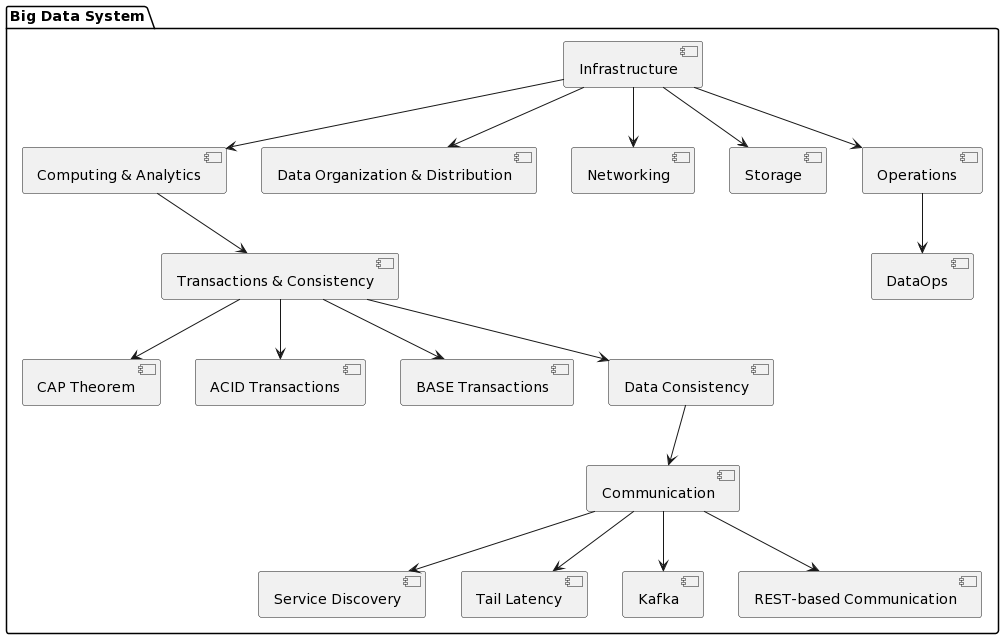
\includegraphics[width=12cm]{media/three-layer-bd.png}
    \caption{A High Level Representation of Big Data Components}
    \label{BDcomponents}
\end{figure}

\begin{thebibliography}{00}


\bibitem{b1} P. Ataei and A. Litchfield, "The State of Big Data Reference Architectures: A Systematic Literature Review," in IEEE Access, vol. 10, pp. 113789-113807, 2022, doi: 10.1109/ACCESS.2022.3217557.
\bibitem{b2} Ataei, Pouya and Litchfield, Alan T., "Big Data Reference Architectures, a systematic literature review" (2020). ACIS 2020 Proceedings. 30.
\bibitem{b3} Framework, D. N. B. D. I. (2015). Draft nist big data interoperability framework: Volume 6, reference architecture. NIST Special Publication, 1500, 6.
\bibitem{b4} Ataei, Pouya and Litchfield, Alan, "Towards a domain-driven distributed reference architecture for big data
systems" (2023). AMCIS 2023 Proceedings. 11.
\bibitem{b5} Dehghani, Z. (2022). Data Mesh. Marcombo


\end{thebibliography}



\end{document}
